\documentclass[xcolor=x11names,compress]{beamer}
\usepackage[utf8]{inputenc}
\usepackage[spanish]{babel}
\usepackage{hyperref}
\hypersetup{colorlinks=true,linkcolor=white}
\usepackage{colortbl}
\usepackage{xcolor}
\usepackage{multirow}
\usepackage{fancyhdr}
\usepackage{graphicx}
\usepackage{framed}
\usepackage[version=0.96]{pgf}
\usepackage{tikz}
\usetikzlibrary{arrows,matrix,shapes,snakes,automata,backgrounds,petri}
\tikzstyle{information text}=[rounded corners, fill=gris]

\newcommand{\figuratikz}[3]
{
\begin{center}%
\begin{figure}[H]%
\begin{minipage}[H]{#1\columnwidth}%
\centering%
\begin{tikzpicture}{node distance=1.3cm,>=stealth',bend angle=45, auto}
{#3}
\end{tikzpicture}
\caption{#2}%
\end{minipage}%
\end{figure}%
\end{center}%
}

\definecolor{shadecolor}{RGB}{243,243,243}
\renewcommand{\figurename}{Figura}

\newtheoremstyle{cuadrado}% name
  {3pt}%      Space above
  {3pt}%      Space below
  {\itshape}%         Body font
  {}%         Indent amount (empty = no indent, \parindent = para indent)
  {\itshape}% Thm head font
  {}%        Punctuation after thm head
  {0em}%     Space after thm head: " " = normal interword space;
        %       \newline = linebreak
  {}%         Thm head spec (can be left empty, meaning `normal')

\theoremstyle{cuadrado}
\newtheorem*{teo}{}


\newcommand{\slidesettitulo}{\textcolor{black}{Suite informática de teoría algorítmica de grafos Graphvisualx}}
\newcommand{\shorttitulo}{Graphvisualx}
\newcommand{\authornombre}{Moisés Gautier Gómez}
\newcommand{\email}{\vspace*{.1in}{
\includegraphics[width=3.5cm]{image.png}}}
\newcommand{\web}{graphvisualx.wordpress.com}
\newcommand{\institucion}{Universidad de Cádiz  \\ Escuela Superior de Ingeniería}
\newcommand{\tutor}{Antonio J. Tomeu Hardasmal}
\newenvironment{fondo}{\begin{teo}}{\end{teo}}



\definecolor{darkgray}{RGB}{237,236,236}
\definecolor{azuladwys}{RGB}{157,189,219}
\definecolor{azuladwys_version}{RGB}{174,208,239}
\definecolor{plata}{RGB}{145,143,144}


\usetheme{Ilmenau}

\setbeamertemplate{footline}{
\begin{tiny}
\setbeamercolor{foot1}{fg=black!70,bg=gray!10}
\setbeamercolor{foot2}{fg=gray,bg=gray!15}
\setbeamercolor{foot3}{fg=gray,bg=gray!10}
\setbeamercolor{foot4}{fg=black!70,bg=gray!20}
\setbeamercolor{foot5}{fg=gray,bg=gray!15}
\setbeamercolor{foot6}{fg=black,bg=gray!20}

%\setbeamercolor{foot1}{fg=azuladwys_version,bg=azuladwys_version}
%\setbeamercolor{foot2}{fg=azuladwys,bg=azuladwys}
%\setbeamercolor{foot3}{fg=azuladwys_version,bg=azuladwys_version}
%\setbeamercolor{foot4}{fg=azuladwys,bg=azuladwys}
%\setbeamercolor{foot5}{fg=azuladwys,bg=azuladwys}
%\setbeamercolor{foot6}{fg=black,bg=gray!20}

% taken from theme infolines and adapted
  \leavevmode%
  \hbox{%
  \begin{beamercolorbox}[wd=.35\paperwidth,ht=2.25ex,dp=1ex,center]{foot1}%
  %\fontsize{5}{5}\selectfont
  \shorttitulo
  \end{beamercolorbox}%
  \begin{beamercolorbox}[wd=.1\paperwidth,ht=2.25ex,dp=1ex,center]{foot2}
  \end{beamercolorbox}%
    \begin{beamercolorbox}[wd=.05\paperwidth,ht=2.25ex,dp=1ex,center]{foot3}
  \end{beamercolorbox}%
    \begin{beamercolorbox}[wd=.25\paperwidth,ht=2.25ex,dp=1ex,center]{foot4}%
  %\fontsize{5}{5}\selectfont
  \web
  \end{beamercolorbox}%
  \begin{beamercolorbox}[wd=.05\paperwidth,ht=2.25ex,dp=1ex,center]{foot5}
  \end{beamercolorbox}%
  \begin{beamercolorbox}[wd=.2\paperwidth,ht=2.25ex,dp=1ex,right]{foot6}%
	\insertframenumber{} / \inserttotalframenumber \hspace*{2ex} 
  \end{beamercolorbox}}%
  \vskip0pt%
\end{tiny}
\vskip10pt
}


%\setbeamertemplate{footline}{}
\setbeamertemplate{navigation symbols}{} %Elimina los iconos que permiten la navegación en el documento

\usecolortheme[named=darkgray]{structure}
\usefonttheme{professionalfonts}
\useoutertheme{miniframes}

\title{\slidesettitulo}
\author{Alumno: \authornombre \\ \email \\ Director: \tutor}
\institute{\institucion}
\date{ }
\setcounter{subsection}{0}

\begin{document}
\scriptsize{



\frame{\frametitle{\textcolor{black}{Gracias}}
Ante todo \ldots
\begin{figure}[H]
\href{Autor: @woodleywonderworks}{
\includegraphics[width=5.5cm]{intro.jpg}}
\end{figure}
}

\frame{\titlepage

}
\section{Presentación}
\subsection{Introducción}

\frame{\frametitle{\textcolor{black}{Todo tiene un comienzo}}

La teoría de grafos, es una rama importante de las matemáticas combinatorias que se ha estudiado intensamente durante cientos de años. Muchas propiedades importantes y útiles de los grafos se han demostrado, sin embargo, otros muchos problemas de mucha complejidad (problemas de complejidad NP o irresolubles en tiempo polinómico) siguen sin resolverse. \newline

La investigación sobre teoría algorítmica de grafos es relativamente reciente. Aunque algunos de los algoritmos fundamentales son viejos, la mayoría de los más destacados han sido descubiertos en las últimas décadas. \newline

}

\subsection{Contexto histórico}

\frame{\frametitle{\textcolor{black}{Primeros tiempos}}

\begin{block}{Historia}
El primer artículo sobre teoría de grafos fue escrito por el famoso matemático suizo Euler, y apareció en 1736. Desde un punto de vista matemático, la teoría de grafos parecía, en sus comienzos, bastante insignificante, puesto que se ocupaba principalmente de pasatiempos y rompecabezas. Sin embargo, avances recientes en las matemáticas y, especialmente, en sus aplicaciones han impulsado en gran medida la teoría de grafos. \\
\end{block}

\begin{figure}[H]
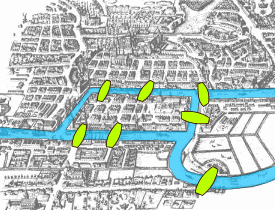
\includegraphics[width=4cm]{konigsberg_bridges.png}
\end{figure}

}

\subsection{Conceptos}

\frame{\frametitle{\textcolor{black}{Generalidad}}

Un grafo es un conjunto de puntos y un conjunto de líneas donde cada línea une un punto con otro.
\begin{fondo}
Llamaremos grafo, G, al par ordenado formado por un conjunto finito no vacío, V, y un conjunto, A, de pares no ordenados de elementos del mismo.\\
\smallskip
\quad V es el conjunto de los vértices o nodos del grafo.\\
\smallskip
\quad A será el conjunto de las aristas o arcos del grafo.\\
\smallskip
Utilizaremos la notación G = (V,A) para designar al grafo cuyos conjuntos de vértices y aristas son, respectivamente, V y A.
\end{fondo}

A cualquier arista de un grafo se le puede asociar una pareja de vértices del mismo. Si $u$ y $v$ son dos vértices de un grafo y la arista $a$ esta asociada con este par, escribiremos $a = uv$.\\

}

\subsection{Estructura de datos}

\frame{\frametitle{\textcolor{black}{Estructura interna}}
Módulos y clases java.

\begin{itemize}
\item Envoltorio: Su estructura interna se basa en un HashMap sobre la que se asentarán todo los grafos del sistema que vayamos creando.
\item CamposNodos y CamposArista: Clases bases para los objetos nodo y aristas del sistema.
\item Algoritmos:Es la encargada de gestionar todos los algoritmos de trabajo de la aplicación.
\item Grafo: Clase envoltorio de la propia clase Envoltorio para facilitar las operaciones con los grafos.
\item LienzoGrafo: Clase encargada de la gestión de los lienzos de trabajo que son objetos de la clase Canvas de AWT.
\item DibujaGrafo: Es la encargada de trabajar con el paquete graphviz y sus ficheros ``.dot'' en la generación de imágenes para los grafos editados o resultantes.
\item Lec\_Esc\_File: Gestiona la lectura y escritura de ficheros que soportan la estructura de datos e información sobre el grafo.
\item Grafico: Módulo que gestiona toda la interacción con el sistema: eventos, estructura de datos, algoritmos e interfaz gráfica. La interfaz visual ha sido creada combinando las bibliotecas Swing y AWT de java.
\end{itemize}

}

\frame{\frametitle{\textcolor{black}{Diagrama de clases}}

\begin{figure}[H]
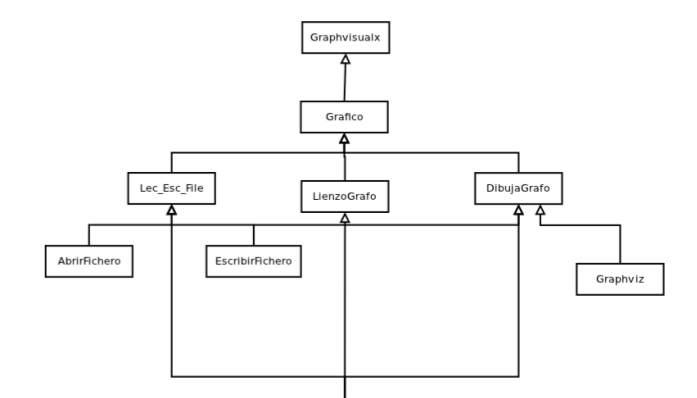
\includegraphics[width=9.75cm]{diag-clases-1.png}
\end{figure}

}

\frame{\frametitle{\textcolor{black}{Diagrama de clases}}

\begin{figure}[H]
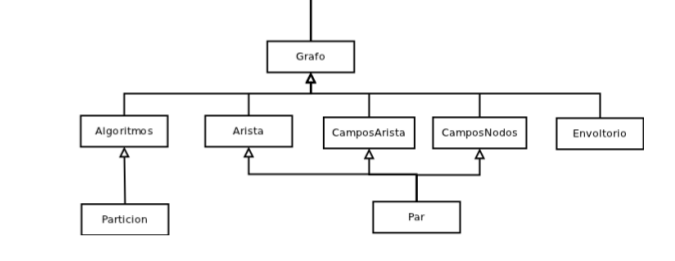
\includegraphics[width=9.75cm]{diag-clases-2.png}
\end{figure}

}


\section{Algoritmos}

\frame{\frametitle{\textcolor{black}{Teoría algorítmica}}

Se analizarán en profundidad todos los algoritmos tratados en el proyecto de fin de carrera intentando en la medida de lo posible una fácil comprensión para el lector falto de conocimientos básicos y para el que tenga unas nociones mayores sobre la materia. \newline

Los algoritmos a tratar serán muy variados:
\begin{itemize}
\item Caminos y Ciclos de Euler.
\item Grafos ponderados.
\begin{itemize}
\scriptsize{
\item Caminos más cortos desde un vértice: Dijkstra.
\item Caminos más cortos desde un vértice: Bellman-Ford.
\item Caminos más cortos: Floyd.
\item Existencia de caminos: Warshall.
\item Árboles de expansión mínimos: Kruskal.
\item Árboles de expansión mínimos: Prim.
}
\end{itemize}
\item Búsqueda en grafos: en profundidad (Depth First Search).
\item Búsqueda en grafos: en anchura (Breadth First Search).
\item Vértice coloración: número cromático.
\item Ordenación Topológica.
\end{itemize}

}

\subsection{Implementación algoritmos}

\frame{\frametitle{\textcolor{black}{Procedimiento}}

Para la implementación de los algoritmos se ha seguido la siguiente metodología de trabajo:
\begin{itemize}
\item Análisis e investigación con diferentes referencias bibliográficas sobre el algoritmo.
\item Una vez realizada un compresión del mismo se realiza una traza para comprobar su funcionamiento.
\item Finalmente se perfila una aproximación en código java para su puesta en prueba con un grafo a través de las distintas clases del sistema.
\end{itemize}

}

\frame{\frametitle{\textcolor{black}{Procedimiento}}

\begin{figure}[H]
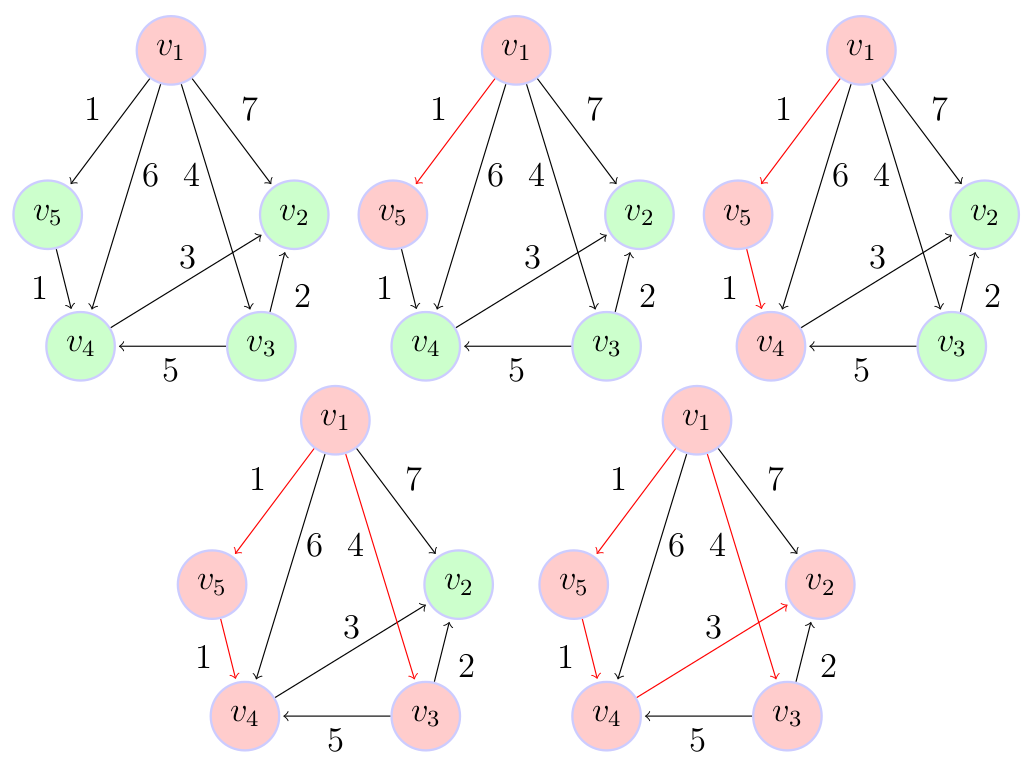
\includegraphics[width=8.5cm]{algoritmo_dijkstra.png}
\end{figure}

}

\frame{\frametitle{\textcolor{black}{Procedimiento}}

\begin{figure}[H]
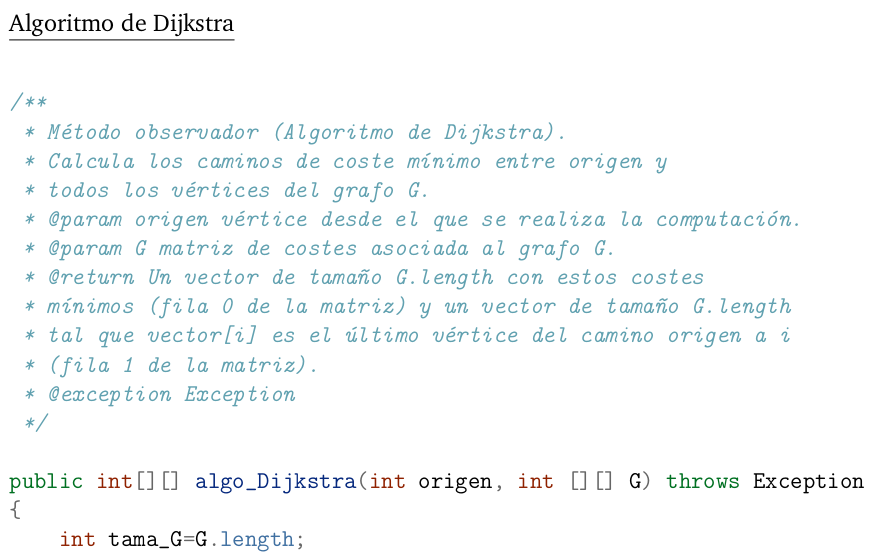
\includegraphics[width=8.5cm]{codigo_1.png}
\end{figure}

}

\section{Planificación temporal}

\frame{\frametitle{\textcolor{black}{Diagrama de Gantt}}

Para la elaboración de este proyecto de fin de carrera me ha sido necesario estudiar de nuevo el funcionamiento de muchos algoritmos sobre grafos que, previamente estudiados durante la titulación, había obviado en ciertos matices que habían que aclarar para acometer con precisión una implementación fina y eficiente.\\ Además, acometer ciertos problemas de programación por eventos, el trabajo con bibliotecas gráficas como AWT y Swing, como empaquetar todo el sistema completo de módulos en un formato ejecutable ``.jar'' ha supuesto una gran demora añadida en muchos puntos del proyecto.\\

\begin{figure}[H]
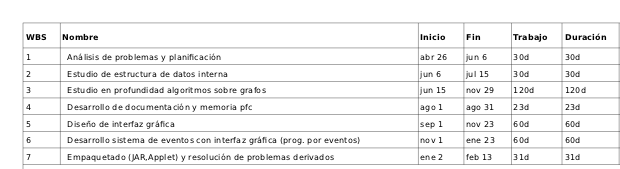
\includegraphics[width=9.5cm]{parte_7.png}
\end{figure}

\centering{\href{http://graphvisualx.forja.rediris.es/planificacion\_graphvisualx/planificacion\_graphvisualx.html}{Planificación}}

}

\frame{\frametitle{\textcolor{black}{Diagrama de Gantt}}

\begin{figure}[H]
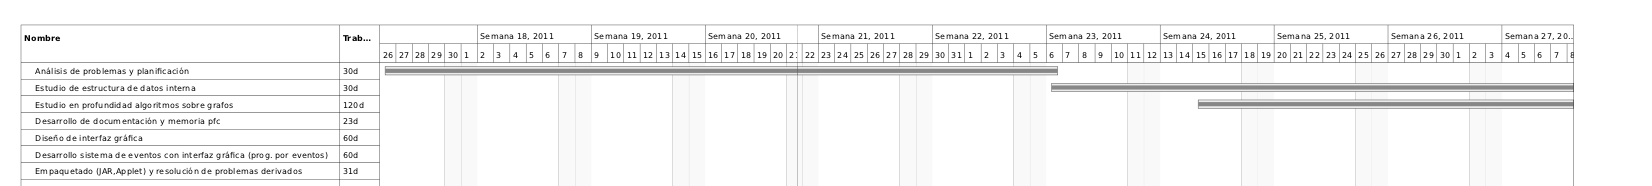
\includegraphics[width=11.5cm]{parte_1_2.png}\\
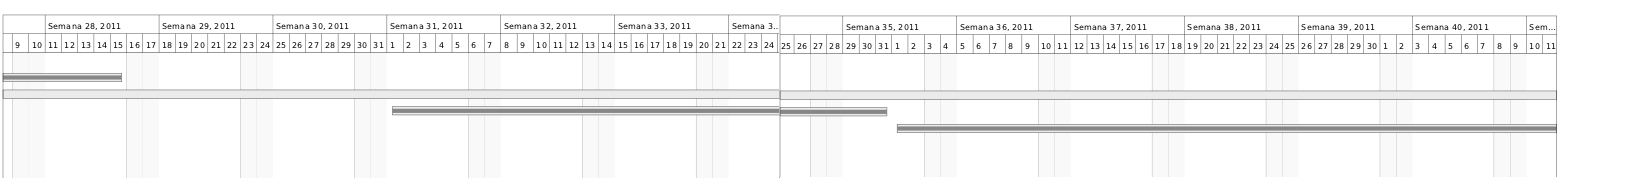
\includegraphics[width=11.5cm]{parte_3_4.png}\\
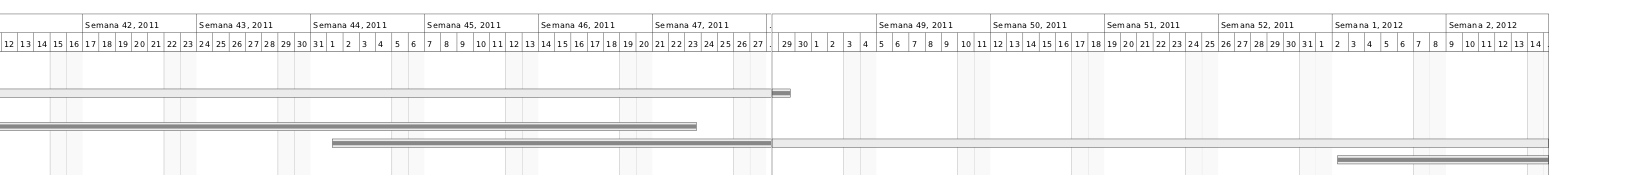
\includegraphics[width=11.5cm]{parte_5_6.png}\\
\end{figure}

}

\subsection{Objetivos}

\frame{\frametitle{\textcolor{black}{Finalidad del proyecto}}

El objetivo es elaborar una aplicación informática que sea capaz de representar un grafo y los posibles algoritmos de procesado que se pueden aplicar a los grafos.

\begin{itemize}
\item Se mostrará en una primera instancia la representación del grafo una vez se haya introducido los valores asociados para las aristas o vértices.
\item Una vez seleccionado el algoritmo de procesamiento o la operación pertinente se mostrará el grafo origen y el resultado de la operación en la misma ventana para resaltar los cambios efectuados por el procesamiento del algoritmo.
\item Habrá un listado con los algoritmos más reseñables de la historia sobre teoría de grafos para aplicar sobre la estructura de grafos creada previamente.
\end{itemize}

Dicha aplicación podría estar enfocada como complemento al material docente de asignaturas de la titulación así como laboratorio de pruebas de algoritmos sobre grafos de ejemplo. También puede utilizarse como soporte ágil para realizar comprobaciones sobre las distintas funcionalidades de los algoritmos disponibles.

}

\section{Aplicación final}

\subsection{Alcance}

\frame{\frametitle{\textcolor{black}{Resultado final}}

El proyecto Suite informática de Teoría Algorítmica de Grafos dará como resultado la aplicación Graphvisualx que cumplirá con todos los objetivos y especificaciones indicados.\newline

La aplicación Graphvisualx se distinguirá en varias partes: el contenido teórico de cada algoritmo a desarrollar como posible comprensión del desarrollo del mismo, el desarrollo de los algoritmos con una entrada ya sea bien en formato fichero o introducida desde la entrada de estándar en el momento de ejecución de la aplicación y contenidos bibliográficos haciendo hincapié en algoritmos clásicos de la materia y su resolución desarrollada.

\begin{figure}[H]
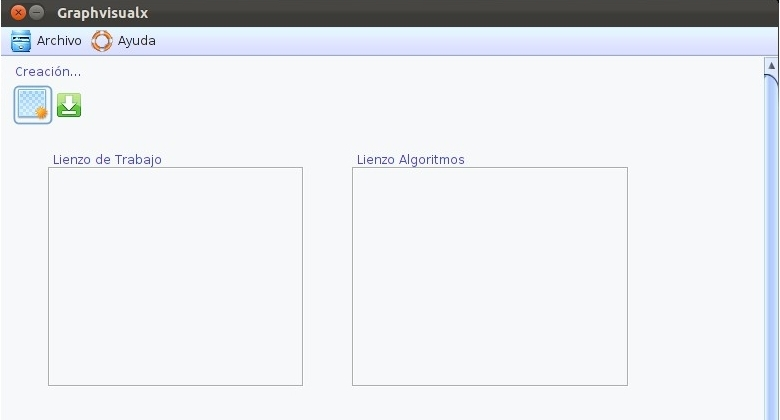
\includegraphics[width=5.5cm]{captura_1.jpeg}
\end{figure}

}

\subsection{Software utilizado}

\frame{\frametitle{\textcolor{black}{Software utilizado}}

En la realización de este proyecto se ha empleado el lenguaje de programación Java (J2SE) en su versión 1.6, empleando además la utilidad de openJDK para dicha plataforma Java.\newline

Para la realización y estructuración del proyecto se ha empleado la herramienta IDE NetBeans v. 7.0.\newline

La documentación y las figuras expuestas en este documento y derivados se han creado mediante el lenguaje de interpretación \LaTeX\ y para las figuras el paquete de opciones de tikz.\newline

La aplicación gráfica Graphvisualx es software libre: usted puede redistribuirlo y / o modificar bajo los términos de la Licencia Pública General de GNU según lo publicado por la Free Software Foundation, ya sea la versión 3 de la Licencia, o (a su elección) cualquier versión posterior.\\
\centering{\href{www.fsf.org}{
\includegraphics[width=2cm]{gplv3.png}}}


}

\frame{\frametitle{\textcolor{black}{Formato de aplicación}}

La aplicación final Graphvisualx estará disponible a través de un fichero \raisebox{0\height}{\href{http://www.oxygen-icons.org/}{
\includegraphics[scale=.15]{JAR.png}}} que será ejecutado desde la distribución favorita del usuario. [Para más información consultar \href{http://graphvisualx.forja.rediris.es/guia\_usuario/guia\_de\_usuario.pdf}{guía de usuario}. (7.7 Ingreso al sistema)] \newline

Además estará disponible una versión en formato Applet en la web para su interacción sin necesitad de instalación de la máquina virtual de java. \newline

\begin{figure}[H]
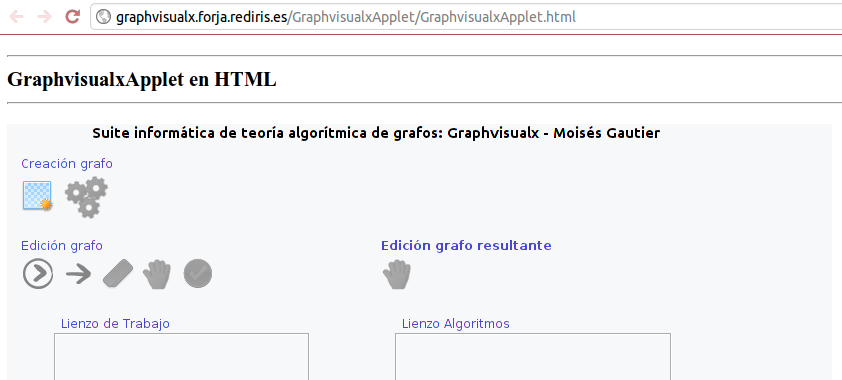
\includegraphics[width=6.5cm]{Graphvisualx-Applet-Recorte.png}
\end{figure}

\begin{center}{\href{http://graphvisualx.forja.rediris.es/GraphvisualxApplet/GraphvisualxApplet.html}{Applet}}\end{center}
}

\section{Guía del usuario}

\frame{\frametitle{\textcolor{black}{Como empezar}}

Una interfaz gráfica de usuario (GUI) presenta un mecanismo amigable al usuario para interactuar con una aplicación. Una GUI proporciona a una aplicación una ``apariencia visual'' única. Al proporcionar distintas aplicaciones en las que los componentes de la interfaz de usuario sean consistentes e intuitivos, los usuarios pueden familiarizarse en cierto modo con una aplicación, de manera que pueden aprender a utilizarla en menor tiempo y con mayor productividad.\\

\begin{figure}[H]
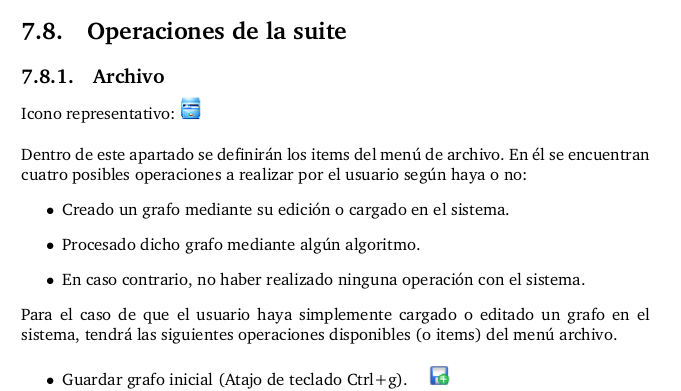
\includegraphics[width=7.5cm]{captura_guia_usuario.png}
\end{figure}


}

\section{Conclusiones}

\frame{\frametitle{\textcolor{black}{Objetivos logrados}}

Durante la realización de la aplicación \emph{Graphvisualx: Suite informática de Teoría Algorítmica de Grafos} como trabajo de fin de carrera, he conseguido profundizar mi conocimiento en estos campos:

\begin{itemize}
\item Ampliación de conocimientos sobre \LaTeX y paquete gráfico PFG-tikz.
\item Profundización sobre el lenguaje java.
\item Aprendizaje sobre programación por eventos.
\item Diseño y creación de interfaces gráficas con el entorno visual de la bibliotecas Swing y AWT de java.
\item Empaquetación de los módulos de lo que se componen el sistema y su obtención final de un fichero ejecutable ``.jar''. Además de la subsanación de problemas derivados de la creación del fichero ejecutable.
\item Aprendizaje sobre herramientas de documentación de clases y generación de estadísticas del sistema de repositorios donde se aloja mi proyecto.
\item Estudio y análisis de nuevos algoritmos de grafos que desconocía.
\item Finalmente, elaboración y empaquetación de la aplicación en formato Applet.
\end{itemize}

}

\frame{\frametitle{\textcolor{black}{Expectativas de futuro}}

El producto obtenido de este proyecto de fin de carrera es un producto final. Por su naturaleza está ideado en principio para la trata y uso de los posibles algoritmos implementados en un principio, dado que no se facilita ningún soporte directo para la implementación de un mayor contenido algorítmico debido a ausencia del mismo o recientes descubrimientos de nuevas teorías algorítmicas. \newline

Se podrían implementar algoritmos de teoría de grafos sobre redes de comunicaciones o relaciones de ontología de la web que dado a la falta de conocimientos en la materia se han obviado para una posible actualización futura. \newline

}

\section{Referencias}

\frame{\frametitle{\textcolor{black}{Referencias}}

\begin{thebibliography}{10} 
\beamertemplatebookbibitems 
\bibitem{1}\color{black}{[BRA, 2008}] 
G. Brassard and P. Bratley. 
\newblock \emph{Fundamentos de algoritmia}, 2008 
\bibitem{2}\color{black}{[ECK, 2002}] 
Eckel Bruce 
\newblock \emph{Piensa en Java}, 2002 
\bibitem{3}\color{black}{[GIB, 1985]}
Alan Gibbons
\newblock \emph{Algorithmic graph theory}, 1985
\bibitem{4}\color{black}{[INT, 2009]}
Thomas H. Cormen
\newblock \emph{Introduction to algorithms 3rd ed.}, 2009
\bibitem{5}\color{black}{[EST, 1998]}
Alfred V. Aho, John E. Hopcroft, Jeffrey D. Ullman
\newblock \emph{Estructuras de datos y algoritmos}, 1998
\bibitem{6}\color{black}{[BER, 1989]}
Claude Berge
\newblock \emph{Graphs}, 1989
\bibitem{7}\color{black}{[GAR, 2003]}
Michael R. Garey, David S. Johnson
\newblock \emph{Computers and intractability: a guide to the Theory of NP-Completeness [26th print.]}, 2009
\end{thebibliography} 
}

\frame{\frametitle{\textcolor{black}{Referencias}}
\begin{thebibliography}{10} 
\beamertemplatebookbibitems 
\bibitem{9}\color{black}{[HAR, 1996]}
Frank Haray
\newblock \emph{Graph theory}, 1996
\bibitem{10}\color{black}{[HOP, 2008]}
John E. Hopcroft, Rajeev Motwani, Jeffrey D. Ullman
\newblock \emph{Introducción a la teoría de autómatas, lenguajes y computación 3ª ed.}, 2008
\bibitem{11}\color{black}{[ROS, 2004]}
Kenneth H. Rosen
\newblock \emph{Matemática discreta y sus aplicaciones}, 2004
\bibitem{12}\color{black}{[LEV, 2007]}
Anany Levitin
\newblock \emph{Introduction to the design \& analysis of algorithms 2nd ed.}, 2007
\bibitem{13}\color{black}{[NEA, 2011]}
Richard Neapolitan, Kumarss Naimipour
\newblock \emph{Foundations of algorithms}, 2011
\bibitem{14}\color{black}{[SED, 2003]}
Robert Sedgewick
\newblock \emph{Algorithms in C++ 3th ed.}, 2003
\bibitem{15}\color{black}{[SKI, 2008]}
Steven S. Skiena
\newblock \emph{The algorithm design manual 2nd ed.}, 2008
\end{thebibliography} 

}



\frame{\frametitle{\textcolor{black}{Final}}
{
\begin{center}
\huge{¿Preguntas?}
\begin{figure}[H]
\href{http://ph03nyx.deviantart.com/}{
\includegraphics[width=2cm]{question.png}}
\end{figure}
\end{center}



Para más información: \href{http://\web}{Página web del proyecto} \newline
Si quieres ir al grano: \raisebox{-.25\height}{
\includegraphics[width=3.5cm]{image.png}}

}
}
\end{document}

